\begin{minipage}{0.55\textwidth}
\begin{align*}
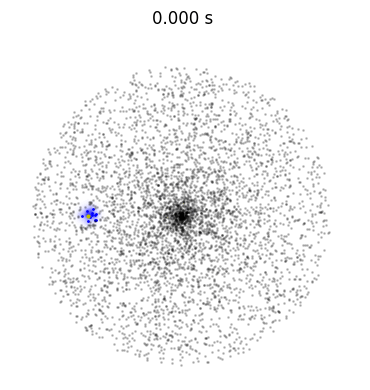
\includegraphics[width=0.49\textwidth]{simulation/2/frame_0.png}\hfill
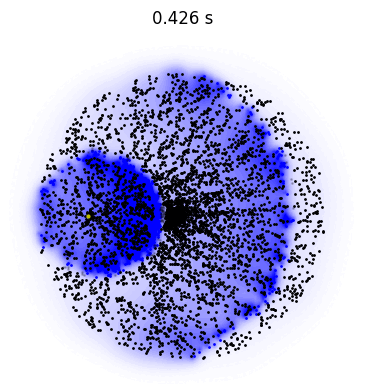
\includegraphics[width=0.49\textwidth]{simulation/2/frame_71.png}
\\[\smallskipamount]
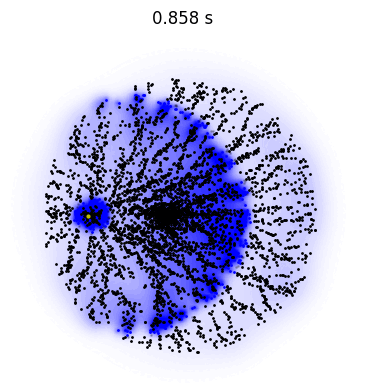
\includegraphics[width=0.49\textwidth]{simulation/2/frame_143.png}\hfill
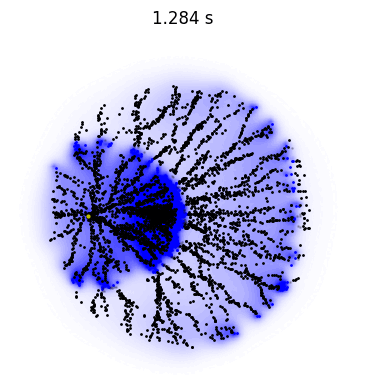
\includegraphics[width=0.49\textwidth]{simulation/2/frame_214.png}
\\[\smallskipamount]
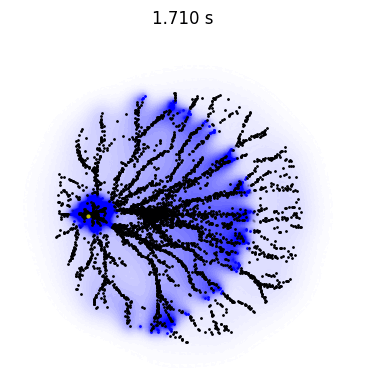
\includegraphics[width=0.49\textwidth]{simulation/2/frame_285.png}\hfill
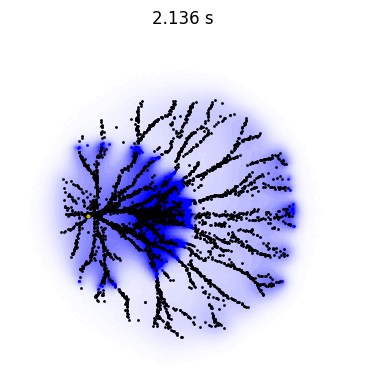
\includegraphics[width=0.49\textwidth]{simulation/2/frame_356.png}
\\[\smallskipamount]
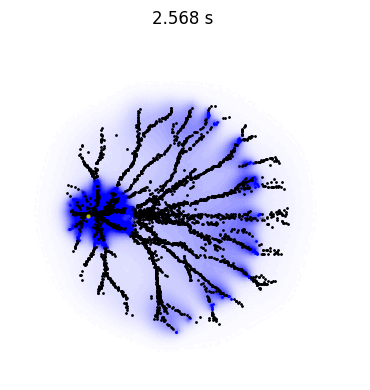
\includegraphics[width=0.49\textwidth]{simulation/2/frame_428.png}\hfill
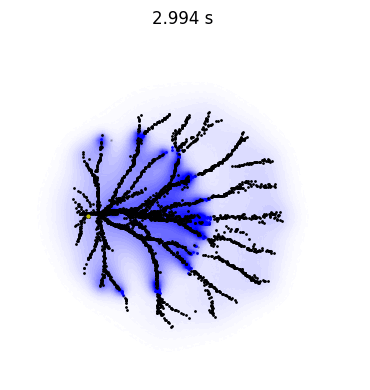
\includegraphics[width=0.49\textwidth]{simulation/2/frame_499.png}
\end{align*}
\end{minipage}
\begin{minipage}{0.45\textwidth}
\subsection{High Density Center}
Here we use a disk with a higher density of particles in its center and an offset pacemaker.
Again a pattern is clearly visible at about $1$s.
The dense center does not seem to affect the spread of the chemical.
After about $2.5$s this high density area transforms into a a slightly thicker, but more or less indistinguishable, branch of the pattern.
\end{minipage}